\documentclass[a4paper,10pt]{article}
%\documentclass[a4paper,10pt]{scrartcl}

\usepackage[utf8]{inputenc}
\usepackage{textcomp}
\usepackage{hyperref}
\usepackage{xcolor}
\usepackage{listings}
\usepackage[cache=false]{minted}
\usepackage{upquote}
\usepackage{graphicx}

\lstset{
  basicstyle=\ttfamily,
  columns=fullflexible,
  frame=single,
  breaklines=true,
  postbreak=\mbox{\textcolor{red}{$\hookrightarrow$}\space},
}

\title{A practical guide to using the AngCor package}
\author{Philip Adsley, iThemba LABS/University of the Witswatersrand\footnote{padsley@gmail.com}\\
Kevin CW Li, iThemba LABS/University of Stellenbosch\\
Harshna Jivan, University of the Witswatersrand\\
Luke Morris, University of York\\
Luna Pellegri, iThemba LABS/University of the Witswatersrand}
\date{\today}

\pdfinfo{%
  /Title    (A pratical guide to using the AngCor package)
  /Author   (Philip Adsley)
  /Creator  ()
  /Producer ()
  /Subject  ()
  /Keywords ()
}

\begin{document}
\lstset{language=bash}
\maketitle

\section{Introduction}

This report contains brief, practically oriented instructions for how to use the various codes contained within the AngCor software package. Most of these codes (everything except the averaging code) have been written by other people. While we (the contributors to this report) may be able to assist users with various parts of the codes, we did not write those codes and so some queries may be beyond our knowledge.

Should you have queries you can e-mail padsley@gmail.com or (preferably) leave a comment on the \href{https://github.com/padsley/AngCorPackage}{Github repository}.

This guide is a {\it living document} and may contain errors, misleading statements or blatent falsehoods. If (when) you find an error please let us know so the guide may be corrected. In addition, if you have any comments, suggestions or corrections, please get in touch so they can be added to the report or (preferably) add them directly on the guide on the Github repository (and please add yourself as an author of the report). The draft version of this report may be found on the Github repository and amended there - please inform Philip of any changes once you are happy with them and the arXiv version of the paper will be updated.

Of particular interest would be other sources of optical-model potentials (if you are the owner of a code to calculate optical-model potentials and would be willing to allow your code to be included within this package or linked to as a submodule then please contact Philip).

A final note of warning - we have used this code for various scenarios for experiments based at iThemba LABS using the K600 magnetic spectrometer and her ancillary detectors. If you are trying to use this code with some other experimental setup at some other place you may have to make some adjustments to the inputs or the averaging code. If you are doing this and you need help, advice or emotional support, please get in touch and we will do what we can to help.

\section{The Physical Problem}

Angular correlations in nuclear reactions are an important tool in helping to assign spins and parities to states, and in properly computing branching ratios for excited states in nuclei by accounting for the missing solid angle in each case. The angular correlations typically depend on the reaction used to populate the state of interest, the spin and parity, and the mode of decay.

To calculate the form of the decay, typically one needs to have the initial spin substate ($m$-state) distribution. This depends on the reaction and, in the present case, comes from the CHUCK3 code. Once the initial $m$-state distribution is known they can be used along with the appropriate decay amplitudes for the reaction of interest to calculate the angular correlations - this is done with the AngCor code.

Finally, in many cases that are investigated with the K600, reactions performed at very forward angles including 0 degrees are used. These reactions typically result in recoiling particles at a wide range of angles, and some smearing of the angular correlation function. This smearing of the angular correlation must be properly accounted for and is done with the averaging portion of the code. This code averages the angcor outputs over the reaction region of interest, weights correctly according to the differential cross section of the initial reaction and produces an averaged (observed) angular correlation function. This averaging code has been written so that the output is in the form of a ROOT TTree, meaning that dynamic gates may be placed on the spectrometer aperture 

Recent experimental studies which have used angular correlations of the type described within this work are:

\begin{enumerate}
 \item studies of the PDR using the K600 and BAGEL, an array of HPGe;
 \item studies of nuclear clustering in light nuclei such as $^{16}$O \cite{dummy} and $^{24}$Mg \cite{dummy} using the K600 and CAKE, an array of silicon detectors \cite{dummy};
 \item studies of $\gamma$-ray transitions within the candidate superdeformed band in $^{28}$Si using the Grand Raiden magnetic spectrometer and CAGRA \cite{dummy}.
\end{enumerate}
  
If you use this software package to calculate angular correlations, please let us know so we can add a reference to the paper in the above list. In addition, if you are willing, please send us the input files that you have used for your calculations - having reference calculations for different examples is extremely helpful for future users.

\section{Package Contents}

The package contains the following pieces of code:

\begin{enumerate}
 \item formf - a code to calculate some monopole and dipole form-factors,
 \item A modified version of CHUCK3, a code for DWBA calculations,
 \item AngCor - a code to calculate angular distributions
 \item AverageAngCorResults - a code to calculate the average (observed) angular distribution given the CHUCK3 and AngCor outputs
 \item TestCalculation.sh - this is an example of how each part of the calculation should run. If you have compiled the codes correctly then you should be able to run this code and produce a test output.
\end{enumerate}

These are introducted code-by-code in the following sections.

In addition, there are a number of shell scripts or other codes within the repository which may be used or modified as required in order to run various parts of the codes. These will be introduced in the relevant section. However, there is one example bash script to introduce now. This code is called TestCalculation.sh and it contains the commands to run each part of the whole package step-by-step. It is included for two reasons - first, so you can test to see if the code is working as expected and second, so you may use it as a guide for running the calculations.

To download the code, one must run the command:\\
\mint[breaklines]{shell-session}|git clone --recurse-submodules https://github.com/padsley/AngCorPackage.git|

which should create a sub-directory called \textquoteleft AngCorPackage\textquoteright inside the directory where you run that command. Inside this new directory are some further subdirectories. At this point, please check that inside the AngCorPackage directory that a directory called AngCorAveraging exists and that it contains files. If it does not, please run the command \mintinline{shell-session}|git pull| within the AngCorAveraging directory.

\section{Optical-model potentials}

Optical-model potentials are not part of this package. As a hint - if you are looking at $\alpha$-particle inelastic scattering then consider using Nolte, Machner and Bojowald (Physical Review C 36 1312). Other optical-model potentials are available. The \href{https://www-nds.iaea.org/RIPL-3/}{RIPL-3 database} is another useful source. At RCNP for $(\alpha,\alpha^\prime)$ reactions a double-folding potential is often used but that code is not included in the present package.

\section{Form Factors}

This code to calculate form factors, formf, was written by M. Harakeh. Details about authorship and the origins of the various form factors may be found in formf.for. The form factors calculated are those of Harakeh and Dieperink \cite{dummy}, Orlandini et al. \cite{dummy} and Satchler \cite{dummy}.

Form factors for monopole and dipole states can be calculated using the code {\it formf}. For this code, the input required is the $\alpha+$nucleus optical model potential. The outputs are form factors which may be used as inputs for CHUCK3 calculations.

The first step here is to compile the code. To do this, go to the {\it formf} directory. Then go into the {\it cio} directory and run the command {\it make}. Then go back up one directory (back to the {\it formf} directory) and run {\it make} again.

An executable {\it formf} should now have been created. The code will then run line-by-line asking for the optical-model potential to be input piece-by-piece. This is worth doing to get to know how {\it formf} works. However, one can also run {\it formf} by giving an input file: \mintinline{shell-session}|./formf < input|.

An example input is:
\newline
\noindent pr\\
140\\
1\\
-18.7776\\
1.57\\
0.58815\\
30\\
.1\\
ex\\

An approximate translation of that input is:
\newline

\noindent pr - Proceed with the calculation\\
140 - Mass of the nucleus\\
1 - Type of the Woods-Saxon potential 1 = volume, 2 = surface\\
-18.7776 - Depth of the WS potential\\
1.57 - Reduced radius for the potential\\
0.58815 - Diffusiveness of the potential\\
30 - Maximum integration radius\\
.1 - Integration step size\\
ex - exit the code\\

It is generally easier to prepare these files beforehand: it is more convinient to use the code in this manner and it is useful to have the old input files available if you are trying to remember what you did some months previously.


\section{CHUCK3}

CHUCK3 is a coupled-channel direct reaction written by Peter Kunz and modified by JR Comfort. CHUCK3 is a coupled-channel code to perform DWBA calculations. Its purpose in the current calculations is twofold. First, it is used to calculate the differential cross section as a function of scattering angle and second, it is used to obtain the substate distribution which is required for AngCor. To do this, a CHUCK3 input file must be prepared. Be careful - these input files are read in with FORTRAN and are thus sensitive to whitespaces and which column quantities are aligned to. It is therefore often much easier to take an existing file and modify it rather than writing one from scratch.

The first step for using CHUCK3 is to compile the code. This should be done by entering the {\it chuck} directory and running the command {\it make}. This should create a {\it chuck} executable.

CHUCK3 is detailed in the instruction manual in the {\it chuck} directory. Note that the version of CHUCK3 in the present case is a modified version of the CHUCK3 code and differs from Kunz's original CHUCK3.

An annotated input is given below - however, please do not try to use it to make an input yourself because \LaTeX\ has likely modified the formatting enough that this will not work. Instead, use the example inputs in {\it chuck/input} as templates. However, a brief note about the form factors - the code {\it formf} gives monopole and dipole form factors. For higher-order cases, one can describe the form-factor in a variety of fashions. However, for the purposes of AngCor it is possible to just use a form factor of one of the reaction potentials.

An example CHUCK3 input is followed by a line-by-line description:

\noindent 11     23000     1    Ca48  136 MeV      ISGDR Excitation\\
100.    0.0    0.15\\
150  2  0 -2\\
0.1     30.\\
136.    4.      2.      48.     20.     1.4\\
  1  1\\
-1.     -100.7  1.25    0.78            -21.4   1.57    0.62 \\
-7.600  4.      2.      48.     20.     1.4\\
  2  2\\
-1.     -100.7  1.25    0.78            -21.4   1.57    0.62 \\
 -2  1  1  0  2  3  0  0 0.10\\
6.      222.49771.25    0.78            37.569061.570   0.62            1.00\\
7.      -967.3841.25    0.78            -247.8991.570   0.62            0.00\\
7.      84.911021.25    0.78            18.198681.570   0.62            2.00\\
-8.     4.71157 1.25    0.78            1.28178 1.570   0.62            1.00\\
            
\noindent 110000023000     1    Ca48  136 MeV      ISGDR Excitation\\
123456789 - these numbers are here to help you line up the ICON values
Options and title for the file. The options are called ICON in the list. In this case, the options are ICON(1)=1 [read additional cards for this run], ICON(2)=1 [according to CHUCK3 documentation this is not used but the modified CHUCK3 code says that this suppresses the printing of form factors if desired], ICON(3-7) are blank or 0\footnote{In order to show the ICON values more clearly, 0s have been added for each blank.}, ICON(8)=2 [Print out scattering amplitudes], ICON(9)=3 [Print out 3-cycle semilog plot of the differential cross section], ICON(10-12)=0 [Don't use relativistic kinematics and turn off a couple of printing options]. \\ \\

\noindent 100.    0.0    0.15\\
Number of angles to calculate (100), starting at $\theta_\mathrm{cm} = 0.0$ in steps of 0.15 degrees.\\

\noindent 150  2  0 -2\\
Use 150 partial waves, with 2 channels the first having $J^\pi = 0^+$ and the second having $J^\pi = 1^-$.\\

\noindent 0.1     30.\\
Integration step size (0.1 fm) and maximum radius for the integration (you shouldn't need to change these but if you're worried about it, try using smaller step sizes and larger radii and seeing if anything changes.\\

\noindent 136.    4.      2.      48.     20.     1.4\\
Lab energy (136 MeV), the mass and charge of the projectile (4 and 2 for $^4$He), target mass and charge (48 and 20 for $^{48}$Ca) and reduced Coulomb charge radius (1.4 fm)\\

\noindent 1  1\\
This defines the channel (number 1). Why the number appears twice is not clear.\\
  
\noindent -1.     -100.7  1.25    0.78            -21.4   1.57    0.62\\
This defines an optical-model potential for the ingoing channel. The (-1) should be split into two parts: 1=a volume Woods-Saxon potential is being defined and the negative sign means that this is the final potential which will be read for this channel. -100.7 MeV, 1.25 fm and 0.78 fm are the depth, reduced radius and diffusivity of the real part of the Woods-Saxon potential, and -21.4 MeV, 1.57 fm and 0.62 fm are the equivalent parameters for the imaginary part.\\

\noindent -7.600  4.      2.      48.     20.     1.4\\
The definition of the second channel. The excited state is at $E_x = 7.6$ MeV, the $\alpha$-particle and $^{48}$Ca definitions remain the same.\\

\noindent 2  2\\
Defines the second channel.\\
  
\noindent -1.     -100.7  1.25    0.78            -21.4   1.57    0.62\\
Again defines a volume Woods-Saxon potential, in this case identical to that given for channel number 1.\\

\noindent -2  1  1  0  2  3  0  0 0.10\\
This line (card) defines the coupling between the two channels. The coupling is from channel 1 to channel 2 (the final channel is given first). The coupling is only in one direction because it is a negative value (-2). The next value (1) defines the orbital angular momentum of the transfer. The next value (0) is twice the value of the spin transferred. The next value is twice the total angular momentum transfer (2). The next value (3) defines the form factor. The following three 0s say ??? and the final value of 0.10 gives the $\beta$ for the calculation. \\
 
\noindent 6.      222.49771.25    0.78            37.569061.570   0.62            1.00\\
First part of the form factor definition. This is a volume form factor of the form $[V(r) + iW(r)] * r^n$. In this case, the parameters for the real and imaginary parts are 222.49771 MeV, 1.25 fm and 0.78 fm, and 37.56906 MeV, 1.570 fm and 0.62 fm respectively. The 1.00 at the end of the line is $n$, the exponent of the factor with $r$.\\

\noindent 7.      -967.3841.25    0.78            -247.8991.570   0.62            0.00\\
Second part of the form factor definition. This is a surface form factor with an $r^n$ component. For this component of the form factor $n=0$.\\

\noindent 7.      84.911021.25    0.78            18.198681.570   0.62            2.00\\
Third part of the form factor definition. This is a surface form factor with an $r^2$ component.\\

\noindent -8.     4.71157 1.25    0.78            1.28178 1.570   0.62            1.00\\
Fourth and final (the 8 which defines the type of the form factor is negative) part of the form factor definition. This is a second-order form factor with an additional $r$ dependence.\\

To run CHUCK3, one should do \mintinline{shell-session}|./chuck < input| to print the output to the screen or \mintinline{shell-session}|./chuck < input > output| to print the output to a file (called output). The output file is a long text file which prints out part of the status for the calculation. Another important file which is generated is the \mintinline{shell-session}|fort.2| file, containing the population of the substates for the scattering at a particular angle.

Please note that the cross section values are required for the averaging code and so you must use CHUCK3 in the form \mintinline{shell-session}|./chuck < input > output| when running CHUCK3 in preparation for doing averaged AngCor calculations.

One particular odd behaviour with CHUCK3 that has been observed is that some calculations will not run unless you have a two blank lines (i.e. carriage returns) at the end of the input file. The reason for this is not entirely understood but if you can see that the outputs are all being read correctly before an error that looks like:\\
\begin{minted}[breaklines]{shell-session}
At line 287 of file chuck.for (unit = 5, file = 'stdin')\\
Fortran runtime error: End of file 
\end{minted}
consider adding a couple of additional lines to the end of the code and trying again. Alternativly, one can try using ICON(1)=9 for the next line which, in theory, should terminate the calculation at the end of the one being performed.

\section{AngCor}

AngCor was written by MN Harakeh and LW Put, with modifications made by M Yosoi and the mysterious RGT.

AngCor calculates the angular correlation function as a function of the polar decay angle ($\theta_{\mathrm{decay}}$) for a reaction involving the scattering of the ejectile at a particular polar scattering angle ($\theta_{\alpha}$ - note that this does not have to be an $\alpha$ particle - it is just a quirk of the naming convention as this code was originally written for use with $\alpha$-particle inelastic scattering reactions with the K600) and azimuthal decay angle ($\phi_{\mathrm{decay}}$).

The first step in using AngCor is to compile the code. This should be done by running \mintinline{shell-session}|make| in the {\it angcor} directory. This should create some object (.o) files and an {\it angcor} executable.

Once this has been done, the angcor calculations may be run. An example input file is given below, followed by an annotated discussion of the input. Note that because angcor must be run for a large number of cases corresponding to various scattering and $\phi_\mathrm{decay}$ angles, some c files for generating the inputs as well as shell scripts for running all of the generated inputs and an awk script for combining the outputs into one large file.

An example AngCor input looks like this:\\


A line-by-line interpretation of the AngCor input is:\\

One peculiarity of AngCor that has been noted is that the particle-particle coincidence option does not seem to produce any output. If you are looking at particle-particle correlations, we have obtained good results using the particle-fission option so we suggest that you use that option.

An example of the generating code for AngCor inputs is {\it make\_input\_010.c}. This code makes AngCor inputs for reactions from a $J^\pi = 0^+$ initial state, to a $J^\pi = 1^-$ excited state followed by an $E1$ decay to a $J^\pi = 0^+$ final state. To run the code, one must first compile it using the command\\ \mintinline{shell-session}|g++ make_input_010.c -o make_input_010|. The code is then run with the command \mintinline{shell-session}|./make_input_010|. This should produce a lot of output files with names similar to {\it input\_ca\_2.1\_4.com}. This particular file will be for $\theta_\alpha = 2.1$ degrees and $\phi_\mathrm{decay} = 4$ degrees.

Once each of the AngCor inputs has been generated in the {\it input} directory, the AngCor calculations may be performed. This may be done using the shell scripts within the {\it input} directory. An example can be found in {\it DoAngCorPR244J\_1.sh} and easily modified to take into account changes to file names. This step may produce a number of errors about IEEE standards - as far as we can tell these are warnings about numerical precision in the compiler but for most of the examples that we have run, the final results are acceptable.

Running all of the AngCor files should take the input {\it .com} files in the {\it input} directory and produce a large number of {\it .lis} files in the {\it output} directory. 

The {\it make\_final.sh} shell script takes the {\it .lis} outputs and combines them into one file. This is done using the {\it sort.awk} script (more on this in a moment) invoked within the {\it make\_final.sh} script. The final output file is comprised of four columns: $\theta_\alpha$, $\theta_\mathrm{decay}$, $\phi_\mathrm{decay}$ and $W(\theta)$. This is the combined AngCor output for all of the various possible polar scattering angles and decay angles. This output file will be used in the averaging portion of the code.

Note that the {\it sort.awk} file which does the combination of the various runs is an inflexible tool. It uses substrings to search for the relevant angles ($\theta_\alpha$ and $\phi_\mathrm{decay}$) for each of the different inputs. Therefore, if you change the number of characters in the names of the output files then you will need to change the size and starting character for the substrings in {\it sort.awk}. Instructions for how to code in awk are beyond the scope of this document but may be easily found online. Additionally, one can add print statements to the awk file to check to see how the substrings are being interpreted. The version of the {\it sort.awk} file which is currently in the respository is designed to use files with names of the form {\it input\_PR244\_J\_1\_1.2\_25.com}.



\section{Averaging the AngCor result}

This part of the code, found in the folder AngCorAveraging was written by P. Adsley based on an archetype code of 'VD' [who is this person Kevin?].

A working ROOT distribution is a prerequisite for using this code. If you don't have ROOT installed and working yet then you need to do that now. Instructions for how to do this may be found on the ROOT website \url{}.

In many cases, the scattering reactions relevant for the current work use finite-acceptance magnetic spectrometers. This means that there is a range of angles which can be populated in the reaction. Especially in the $0-2$ degree range for the K600 aperture, this can result in a range of recoil angles over tens of degrees for the recoil. Therefore, the results of the AngCor calculations need to be smeared over the finite aperture size of the spectrometer.

In order to run this code, one needs to first modify the code and then to compile it. The modifications are mainly in file AverageAngCorResults.h - one needs to ensure that the correct number of points are set for $\theta_\alpha$ (NumberThetaAlphaPoints) - one must set this value to various different options but the easiest solution is to make it the same as the number of angles that one used in the CHUCK3 calculation. Another variable (ThetaAlphaStartAngle) is provided for setting the initial angle for the DWBA calculations if for some reason the calculations were performed starting at an angle greater than 0\textdegree. The value of DeltaThetaAlpha should be set to be the size of the increment on the angles in the CHUCK3 input file. The number of $\phi_\alpha$ points (NumberPhiAlphaPoints) can remain 360. The number of $\theta_\mathrm{decay}$ points (NumberThetaDecayPoints) should be the same as the number of points that one used in the AngCor input file. The number of $\phi_\mathrm{decay}$ points (NumberPhiDecayPoints). Finally, the number of CHUCK3 angles (NumberOfCHUCK3Angles) should be set to be the number of angle points which one used when running the CHUCK3 code.

If some of these values are set incorrectly then it is very possible that either the angular correlation produced will be incorrect or alternatively that the code will crash because the code will go beyond the end of an array while trying to store the cross section or AngCor data.

To compile, one needs to run the command:

\begin{minted}[breaklines]{shell-session}
g++ AverageAngCorResults.cpp -o AverageAngCorResults `root-config --cflags --libs` 
\end{minted}

The code requires three arguments to run. You can find these out by running \mintinline{shell-session}{./AverageAngCorResults} with no arguments which will return the output: \mintinline[breaklines]{shell-session}{usage: mcerr <filename for cross section> <filename for AngCor results> <filename for output>}. The file for the cross section will be the file which was created in the command \mintinline[breaklines]{shell-session}{./chuck3 < input > output.} For the AngCor results use the combined file created when running the \mintinline{shell-session}{make_final.sh} shell script. Note that one needs to also give the path for the input files if they are not within the current directory.
 
To get the angular correlation function in the centre-of-mass frame of the colliding system one can use the \mintinline{shell-session}{TTree} which was output in the ROOT file. In order to plot the ACF, one should run a command of the form:
\mint[breaklines]{cpp}{AngCorData->Draw("ThetaDecayCM>>hW(181,0,180)","Weight*(CUTS)");}

This will weight the $\theta_{\mathrm{decay}}$ distribution with the correct weight which is derived from the information on the differential cross section from CHUCK3 and the angular correlation functions from AngCor. An example (GenerateOutputAngularCorrelation.cpp) of how to do this is given in the {\it AverageAngCorResults} directory. The resulting plot should look something like Figure \ref{fig:2plusTo0PlusAlphaEmission}.

\begin{figure}
 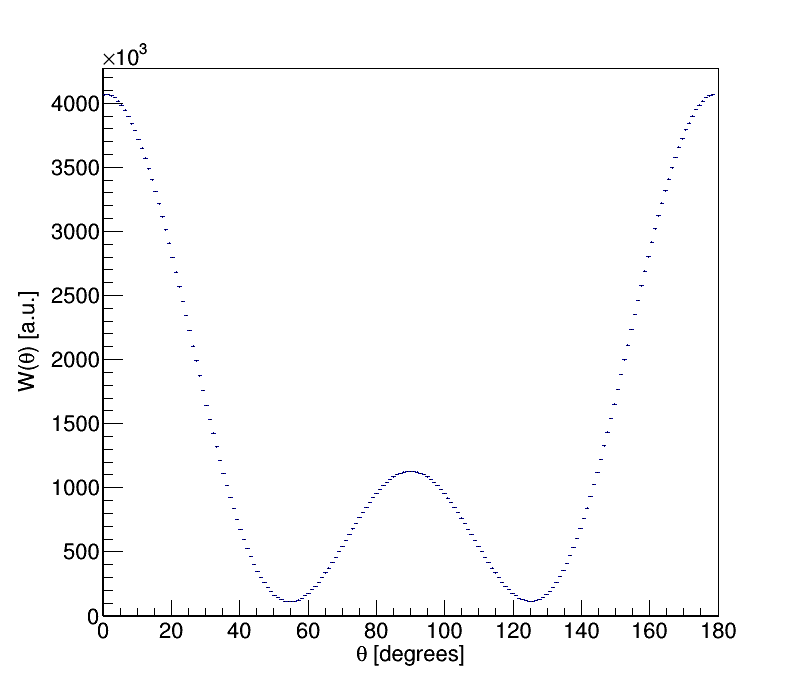
\includegraphics[width=\textwidth]{QuadrupoleAlphaDecayExample.png}
  \caption{Angular correlation function for $J^\pi = 2^+$ to $J\pi = 0^+$ decay from a state populated in the $^{24}$Mg($\alpha,\alpha^\prime$)$^{24}$Mg reaction.}
  \label{fig:2plusTo0PlusAlphaEmission}
\end{figure}


Note that, at the moment the code does {\it \bf not} provide information on the lab angles of the decaying particles. The calculation of this value is a work in progress and will be added when available.

\section{Acknowledgements and Thanks}

None of this work would have been possible without Muhsin Harakeh, both for providing the codes in the first place and for allowing us to put them online. Any mistakes found in this brief guide are solely the responsibility of the authors.

\bibliography{AGuideToAngCor}
\end{document}
